\documentclass{beamer}
\usepackage[utf8]{inputenc}

\usepackage{utopia} %font utopia imported

\usetheme{Madrid}
\usecolortheme{default}

%------------------------------------------------------------
%This block of code defines the information to appear in the
%Title page
\title[CLI-DOS] %optional
{CLI-DOS: Collaborative Counteraction against Denial of Service in the Internet of Things}

\subtitle{Status, Main Results and Plan}

\author[Atiiq, Syafiq Al] % (optional)
{Syafiq Al Atiiq\inst{1} \and Christian Gehrmann\inst{1}}

\institute[LTH] % (optional)
{
  \inst{1}%
  Dept. of Electrical and Information Technology\\
  LTH Lund University
}

\date[WS 2019] % (optional)
{Sec4Factory Workshop, October 2019}

\logo{
\includegraphics[height=1cm]{lth-logo.jpg}}

%End of title page configuration block
%------------------------------------------------------------



%------------------------------------------------------------
%The next block of commands puts the table of contents at the 
%beginning of each section and highlights the current section:

\AtBeginSection[]
{
  \begin{frame}
    \frametitle{Table of Contents}
    \tableofcontents[currentsection]
  \end{frame}
}
%------------------------------------------------------------


\begin{document}

%The next statement creates the title page.
\frame{\titlepage}


%---------------------------------------------------------
%This block of code is for the table of contents after
%the title page
\begin{frame}
\frametitle{Table of Contents}
\tableofcontents
\end{frame}
%---------------------------------------------------------


\section{Background}

%---------------------------------------------------------
%Changing visivility of the text
\begin{frame}
\frametitle{Background}

\begin{itemize}
    \item<1-> IoT devices are especially exposed to the Denial of Service attack.
    \item<2-> It is even harder to defend DoS in IoT environment, due to:
    \begin{itemize}
    \item Limited resource (CPU and memory).
    \item Transmission capabilities.
    \item Limited battery.
    \end{itemize}
    \item<3-> Denial of Service (DoS) in IoT
    \begin{itemize}
	\item Flooding a server hosts with messages.
	\item Exhaust server resources (e.g. bandwidth, processing, energy)
	\item Less reactive or even unable to serve legitimate requests    
    \end{itemize}
    \item<4-> Countermeasure categories: router-based and host-based.
\end{itemize}
\end{frame}

%---------------------------------------------------------

\section{Current Approach}

%---------------------------------------------------------
%Changing visivility of the text
\begin{frame}
\frametitle{Current Approach}
Existing mechanisms only either:
\begin{itemize}
    \item<1-> Make it more difficult to perform massive scale DoS attacks, or...
    \item<2-> Completely shut down the connection from outside world to save energy
\end{itemize}
\end{frame}

%---------------------------------------------------------

\section{Proposal}

%---------------------------------------------------------
%Changing visivility of the text
\begin{frame}
\frametitle{CLI-DOS}
A Collaborative Counteraction against Denial of Service. \pause \\
The rationale:
\begin{itemize}
	\item<1-> Reducing the impact of DoS attacks against a victim device, and
	\item<2-> Offloading a computational expensive filtering at the IoT unit to a much more powerful gateway, while at the same time...
	\item<3-> Allowing legitimate request to be served to the best possible extent
\end{itemize}
\end{frame}

\begin{frame}
\frametitle{CLI-DOS(Scenario)}
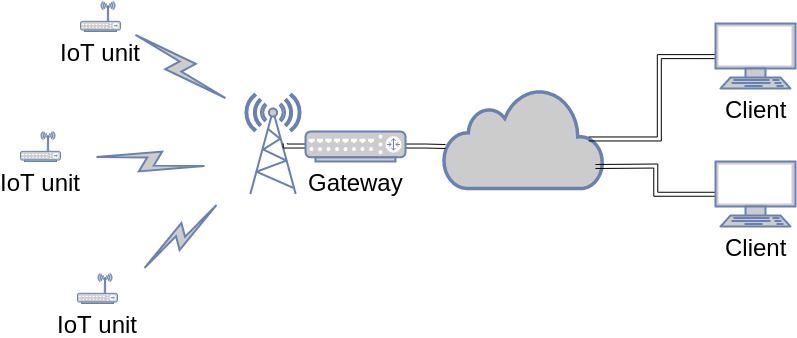
\includegraphics[height=4.3cm]{gambar/default.jpg}
\\
A resource-constrained, wireless IoT-units are connected and able to serve requests.
\end{frame}

\begin{frame}
\frametitle{CLI-DOS}
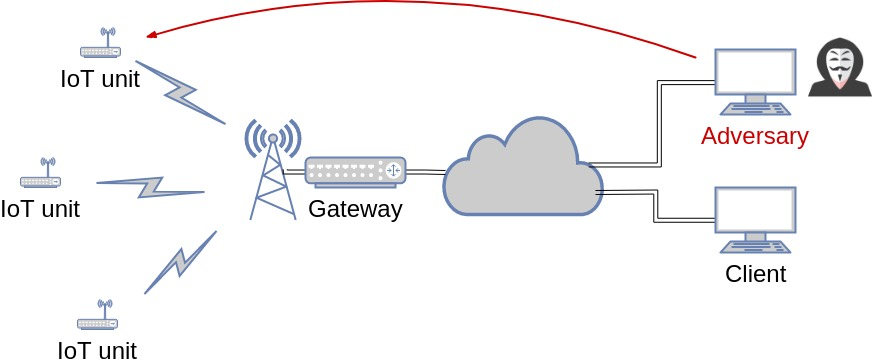
\includegraphics[height=4.3cm]{gambar/adv.jpg}
\\
An adversary repeatedly send bogus messages to the IoT units, trying to induce the device to worthlessly commit resources.  
\end{frame}

\begin{frame}
\frametitle{CLI-DOS}
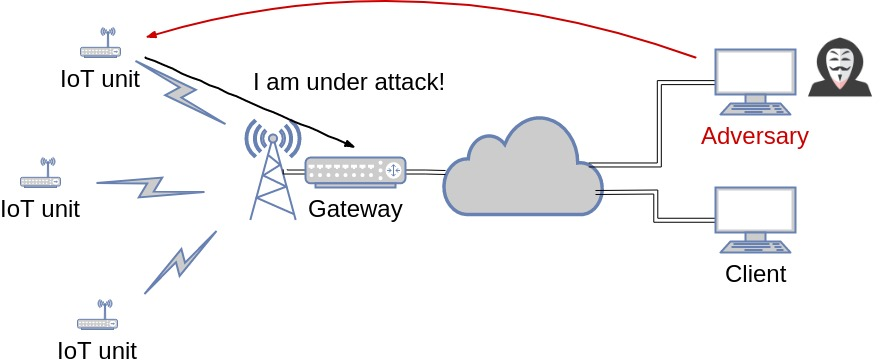
\includegraphics[height=4.3cm]{gambar/inform.jpg}
\\
The IoT unit send a request to the gateway to start a security filtering mechanism, i.e. block ranges of IP, block all traffic but CoAP, etc. The request also contains time $S$ as a sleeping period (victim server shutting down the radio communication).   
\end{frame}

\begin{frame}
\frametitle{CLI-DOS}
To distinguish the valid and invalid messages, the victim uses a short MAC (Message Authentication Code)\footnotemark embedded in token field of the CoAP.

Default CoAP packet format: \\
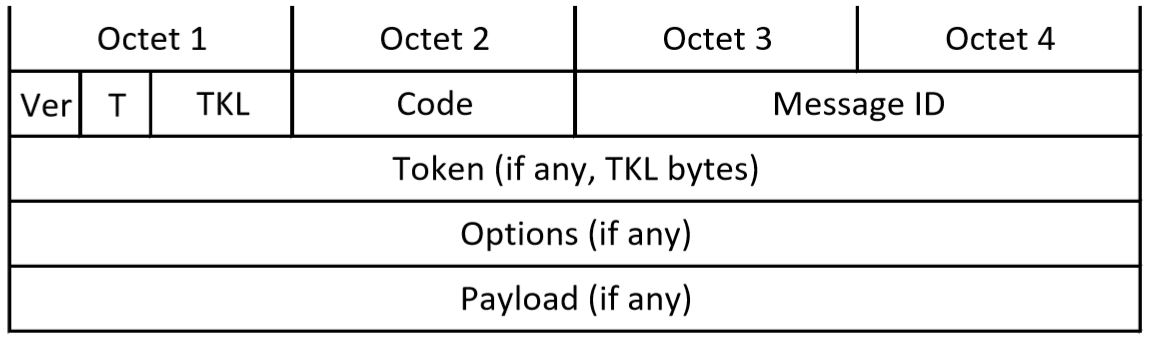
\includegraphics[height=2.05cm]{gambar/coap_format.jpg} \\

CoAP with short MAC: \\
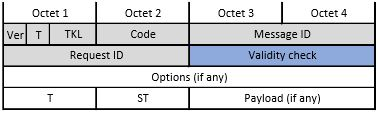
\includegraphics[height=2.1cm]{gambar/coap_adaptive.jpg}

\footnotetext{\tiny{C. Gehrmann, M. Tiloca and R. Höglund, "SMACK: Short message authentication check against battery exhaustion in the Internet of Things"}}
\end{frame}

\begin{frame}
\frametitle{CLI-DOS}
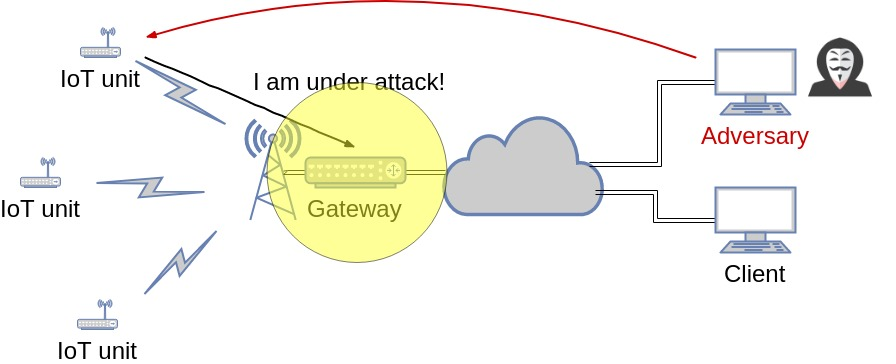
\includegraphics[height=4.3cm]{gambar/proc.jpg}
\\
The gateway now: 
\begin{itemize}
\item Proceses the received information to calculate a new filtering rule. 
\item Measure the number of valid/invalid packets targetting the victim.
\item Store the valid packet in internal buffer.
\end{itemize}
\end{frame}

\begin{frame}
\frametitle{CLI-DOS}
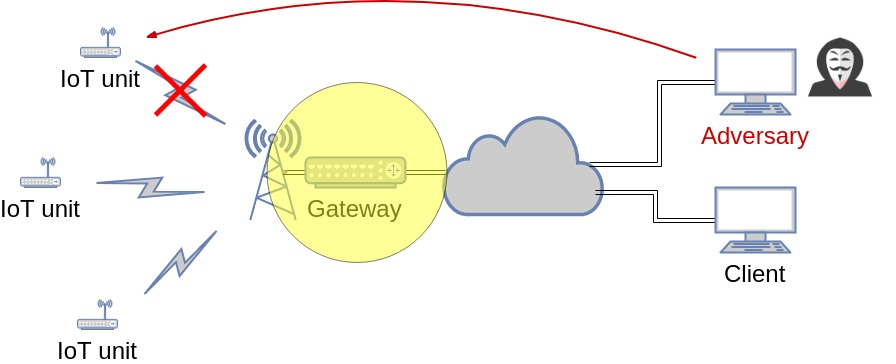
\includegraphics[height=4.3cm]{gambar/off.jpg}
\\
The IoT unit goes into sleep mode and only comes into active mode after agreed sleep period $S$.
\end{frame}

\begin{frame}
\frametitle{CLI-DOS}
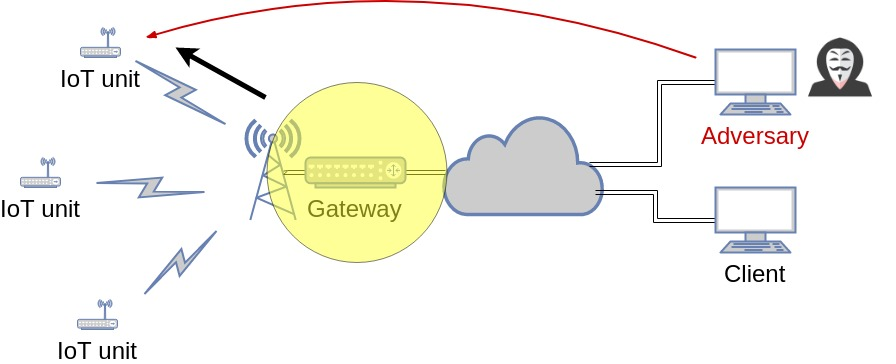
\includegraphics[height=4.3cm]{gambar/back.jpg}
\\
After sleep period $S$ is over, if invalid messages are below threshold, the gateway forwards all the packets from the buffer. Otherwise, the gateway updates its filtering rule to a more restrictive setting without forwarding any packets to the IoT unit. If it still continue, it sends a general warning to the system responsible.
\end{frame}
%---------------------------------------------------------

\section{Status}

%---------------------------------------------------------
%Changing visivility of the text
\begin{frame}
\frametitle{Status}

\includegraphics[height=1cm]{gambar/contiki.png}      
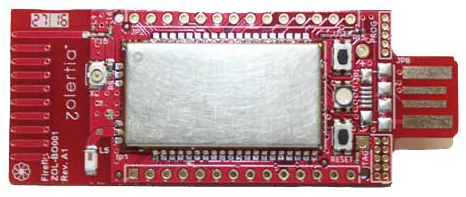
\includegraphics[height=1.5cm]{gambar/firefly.png}
\begin{itemize}
\item<1-> Implemented as an additional module for Contiki-NG.
\item<2-> Hardware for testing: Zolertia Firefly rev.A.
\item<3-> Experimental evaluation on a local testbed.
\end{itemize}
\end{frame}

\begin{frame}
\frametitle{Experimental Evaluation (On progress)}
Measured values:
\begin{itemize}
\item Round Trip Time.
\item Energy usage.
\end{itemize}

Variation of:
\begin{itemize}
\item Attack intensity
\item Number of clients
\item Gateway policies
\end{itemize}
\end{frame}

\begin{frame}
\frametitle{The End}
Thank you! Questions?
\end{frame}

%---------------------------------------------------------


\end{document}